\documentclass{article}

\usepackage[utf8]{inputenc}
\usepackage{amsmath}
\usepackage{amssymb}
\usepackage[margin=2cm]{geometry}
\usepackage{graphicx}

\newcommand{\R}{\mathbb{R}}
\newcommand{\PR}{\mathbb{P}}
\newcommand{\N}{\mathbb{N}}
\newcommand{\C}{\mathbb{C}}
\newcommand{\Z}{\mathbb{Z}}

\renewcommand{\mod}{\,\mathrm{mod}\,}

\setlength{\parindent}{0px}

\begin{document}

\section{Collatz-Problem}

\subsection{Ablauf der Zahlenfolge}
Suche dir eine zufällige Zahl $n \in \N \setminus \{0\}$
\begin{enumerate}
\item Wenn $n \mod 2 = 0 \rightarrow n$ nimmt $\frac{n}{2}$ an
\item Wenn $n \mod 2 = 1 \rightarrow n$ nimmt $3n + 1$ an
\item Vorgang wiederholen
\end{enumerate}

\subsection{Beispiele}
$5 \rightarrow 16 \rightarrow 8 \rightarrow 4 \rightarrow 2 \rightarrow 1 \rightarrow 4 \rightarrow \, ... $ (ungerade Zahl mit den wenigsten Schritten)\\
$8 \rightarrow 4 \rightarrow 2 \rightarrow 1 \rightarrow 4 \rightarrow \, ...$

\subsection{Folgerung}
Jede mögliche Zahl endet im Folgeschema $4 \rightarrow 2 \rightarrow 1 \rightarrow \, ...$ \\
Aber: Nicht beweisbar

\subsection{Statistiken}
[Statistiken einfügen]


\subsection{Collatz-Graph einer Funktion}
$f: \N \mapsto \N$ bildet den Collatz-Graphen einer zahlentheoretischen Funktion ab. 

\subsubsection{Nachfolgerabbildung}

Die einfachste dieser Funktionen ist die Nachfolgerabbildung
\[s: \N \mapsto \N; \, s(n) = n + 1\]

\section{Probleme mit 0}
\subsection{Teilen durch 0}
\subsubsection{Grenzwertbetrachtung}
Durch die Definition einer Funktion $f(x) = \frac{n}{x}$ für eine beliebige Zahl $n \in \N \setminus \{0\}$
\begin{align*}
\lim\limits_{\underset{x < 0}{x \to 0}} \frac{n}{x} &= - \infty \\
\lim\limits_{\underset{x > 0}{x \to 0}} \frac{n}{x} &= + \infty \\
\lim\limits_{\underset{x < 0}{x \to 0}} \frac{n}{x} &\neq \lim\limits_{\underset{x > 0}{x \to 0}} \frac{n}{x}				\\
- \infty &\neq + \infty											\\
\Longrightarrow \frac{n}{0} &= n. d.
\end{align*}

\subsection{0 als Potenzbasis mit 0 im Exponenten}
\subsubsection{Grenzwertbetrachtung}

\begin{align*}
\lim\limits_{\underset{x > 0}{x \to 0}} x^x &= 1 \\
\Longrightarrow 0^0 &= 1 \\
\end{align*}

\subsubsection{Reversibles potenzieren}

\begin{align*}
5^3 &= \frac{5^4}{5} = 5 \cdot 5 \cdot 5 = 125 	\\
5^2 &= \frac{5^3}{5} = 5 \cdot 5 = 25 			\\
5^1 &= \frac{5^2}{5} = 5 = 5 					\\
5^0 &= \frac{5}{5} = 1 							\\
0^0 &= \frac{0}{0} = n.d.
\end{align*}

\section{Primzahlen}
\subsection{Definition}

Für eine natürliche Zahl $N \in \N \setminus \{0\,;\,1\}$ gilt $N \in \PR$, wenn für jede Zahl $n_j \in \N \setminus \{0\,;\,1\,;\,N\}$ gilt:
\[ N \mod n_j \neq 0\]

\subsection{Erschließung/Errechnung}

\subsubsection{Mersennesche Zahlen}

Für eine Zahl $N \in \N$ der Form
\[ N = 2^n - 1;\, n \in \N\]
kann $N \in \PR$ nur dann gelten, wenn $n \in \PR$ gilt. \\

$\Longrightarrow$ Zahlen der Form
\[ M_p := 2^p - 1; \, p \in \PR \]
heißen $Mersennesche\,Zahlen$, die allerdings nicht zwingend Teil der Menge $\PR$ sind.

\subsubsection{Beispiele für Mersennesche Primzahlen}

\begin{align*}
M_2 &= 2^2 - 1 = 3		\\
M_3 &= 2^3 - 1 = 7		\\
M_5 &= 2^5 - 1 = 31		\\
M_7 &= 2^7 - 1 = 127	\\
\end{align*}

\subsubsection{Beispiele für Mersennesche Nicht-Primzahlen}
\begin{align*}
M_{11} &= 2^{11} - 1 = 23 \cdot 89 = 2047			\\
M_{23} &= 2^{23} - 1 = 47 \cdot 178481 = 8388607
\end{align*}

\subsubsection{Fermatsche Zahlen}

Für eine Zahl $N \in \N$ der Form
\[ N = 2^n + 1;\, n \in \N \]
kann $N \in \PR$ nur gelten, wenn $n = 2^m;\, m \in \N$ gilt.

$\Longrightarrow$ Zahlen der Form
\[ F_n := 2^{2^n} + 1\]
heißen $Fermatsche\,Zahlen$, die allerdings nicht zwingend Teil der Menge $\PR$ sind.

\subsubsection{Beispiele für Fermatsche Primzahlen}

\begin{align*}
F_1 &= 2^{2^1} + 1 = 2^{2} + 1 = 5		\\
F_2 &= 2^{2^2} + 1 = 2^{4} + 1 = 17		\\
F_3 &= 2^{2^3} + 1 = 2^{8} + 1 = 257	\\
F_4 &= 2^{2^4} + 1 = 2^{16} + 1 = 65537	\\
\end{align*}

\subsubsection{Beispiel für Fermatsche Nicht-Primzahlen}
\begin{align*}
F_5 &= 2^{32} + 1 = 641 \cdot 6700417 = 4294967297 \\
F_6 &= 2^{64} + 1 =  274177 \cdot 67280421310721 = 1,844674407 \cdot 10^{19}
\end{align*}

\section{Riemannsche Vermutung}

\subsection{Pifunktion}
Die Pifunktion $\pi(x)$ beschreibt für $x_n$ die Anzahl an Primzahlen, die Teil des Intervalls $[0;\,x_n]$ sind.

\subsubsection{Näherungen}
\[ \frac{x}{\ln(x)} \]
\[ \textrm{li}(x) = \int\limits_{0}^{x} \frac{\textrm{d}\,t}{\textrm{ln}\,t} \]
\\
\begin{center}
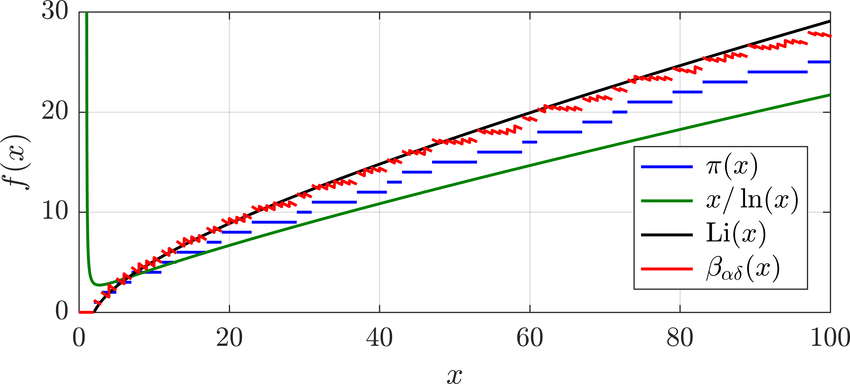
\includegraphics[width=0.5\textwidth]{prime-counting.png}
\end{center}
$\Longrightarrow$ Asymptotisch äquivalent

\subsection{Primzetafunktion}

\subsection{Riemannsche Zetafunktion}

Für eine Zahl $s \in \C; \textrm{Re}(s) > 1$ gilt:
\begin{align*}
P(s) &= \sum\limits_{p \in \mathbb{P}} \frac{1}{p^s} \\
P(s) &= \textrm{log}(\zeta(s))
\end{align*}

\subsubsection{Eulersche Produktformel}
Für alle $z \in \C$ mit $Re(z) > 1$ gilt
\[ \zeta(z) = \prod_{p \in \PR} {\frac{1}{1 - \frac{1}{p^z}}}  = \sum_{n=1}^{\infty} \frac{1}{n^z}\]
$Beweisidee:$ Für eine feste Primzahl $p \in \PR$ kann der Faktor in obigen Produkt in eine geometrische Reihe
\[ \frac{1}{1 - \frac{1}{p^s}} = \sum_{n=0}^{\infty} {\frac{1}{p^{nz}}} \]
entwickelt werden. Wenn also $p_1, p_2, ... p_n$ die ersten $n$ Primzahlen sind, so ist

\begin{align*}
\prod_{k=1}^{n} {\frac{1}{1 - \frac{1}{{p_k}^z}}} &= \sum_{k_1=0}^{\infty} {\frac{1}{{p_1}^{k_1 z}}} \cdot \sum_{k_2=0}^{\infty} {\frac{1}{{p_2}^{k_2 z}}} \cdot\cdot\cdot \sum_{k_n=0}^{\infty} {\frac{1}{{p_n}^{k_n z}}} \\
&= \sum_{k_1=0}^{\infty} \cdot\cdot\cdot \sum_{k_n=0}^{\infty} \frac{1}{({p_1}^{k_1} \cdot\cdot\cdot {p_n}^{k_n})^z} \\
&= \cdot\cdot\cdot
\end{align*}
\subsubsection{Zetafunktion für negative Werte}

Für alle $z \in \C$ mit $\textrm{Re}(z) < 0$ gilt
\[ \zeta(1-z) = \pi^{-z} \cdot 2^{1-z} \cdot \Gamma(z) \cdot\left(\frac{\pi z}{2}\right) \cdot \zeta(z) \]
Außerdem ist die Gammafunktion durch 
\[ \Gamma(z) = \lim\limits_{n \to \infty} \frac{n! \cdot n^z}{\prod\limits_{k=0}^{\infty} (z+k)} \]
definiert.

\subsubsection{Triviale Nullstellen}
Triviale Nullstellen $N_j$ sind solche, für die $\textrm{Re}(N_j) < 0$, $\textrm{Im}(N_j) = 0$ und $N_j \mod 2 = 0$ gilt.

\subsubsection{Komplexe Nullstellen}
Komplexe Nullstellen $N_j$ sind solche, für die $\textrm{Re}(N_j) = \frac{1}{2}$ gilt.

\subsubsection{Vermutung}
\begin{itshape}
Es gibt keine Nullstellen anderer Art und alle nichttrivialen Nullstellen der Zetafunktion liegen auf einer Geraden parallel zur imaginären Achse.
\end{itshape}
\\
Aber: Nicht bewiesen \\
\\
\begin{center}
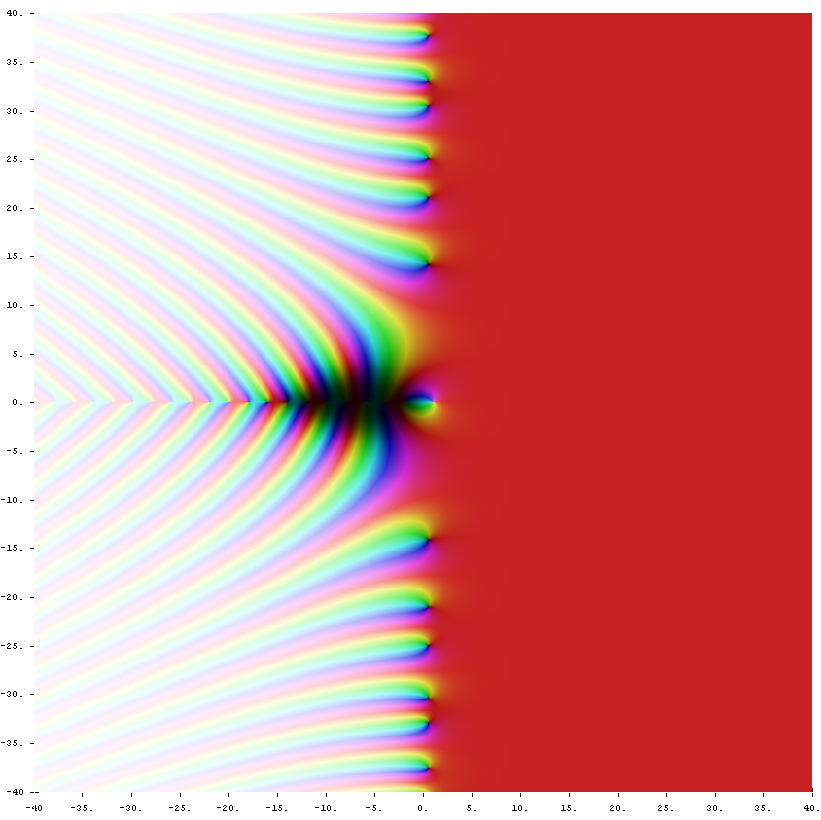
\includegraphics[width=0.5\textwidth]{complex_zeta.jpg}
\end{center}

\end{document}
